\documentclass[11pt]{scrreprt}

\usepackage[T1]{fontenc}
\usepackage[utf8]{inputenc}
% \usepackage[ngerman]{babel}

\usepackage{graphicx}
\graphicspath{ {imgs/} {../evaluation/graphbrain_semsim/case_studies/plots/}}

\usepackage[backend=biber, style=alphabetic]{biblatex}
%\usepackage[backend=bibtex, style=authoryear-comp]{biblatex}
%\newcommand{\citep}{\parencite}  % adds \citep alias for citing with parenthesis
\addbibresource{MA.bib}


\KOMAoptions{parskip=full}

\usepackage{amsmath}
%\usepackage{parskip}
\usepackage{hyperref}
\usepackage{caption}
\usepackage{subcaption}
\usepackage{booktabs}
\usepackage{rotating}


\usepackage{array}  % needed for '\newcolumntype' command
\newcolumntype{L}[1]{>{\raggedright\arraybackslash}p{#1}}  % define "L" column type


\usepackage{newfloat}
\DeclareFloatingEnvironment[
  listname = {List of Patterns} ,
  name = Pattern,
  placement = h,
  within = none
]{pattern}

%\let\textsf\undefined
%\newcommand{\textsf}[1]{\normalfont\sffamily #1}}}
%\newcommand{\textsfs}[1]{{\small{\normalfont\sffamily #1}}}
%\newcommand{\textsft}[1]{{\tiny{\normalfont\sffamily #1}}}


\usepackage{lipsum}  % produces dummy text


\begin{document}


% ========== Title page

\titlehead
{
\begin{tabular}{ll}
\begin{minipage}{0.5\textwidth}
	\textbf{Technische Universität Berlin} \\
	Fakultät IV: Elektrotechnik und Informatik \\
	Institut für Telekommunikationssysteme \\
	Fachgebiet Verteilte offene Systeme	
\end{minipage}
&
\begin{minipage}{0.5\textwidth}
	\raggedleft
	
\includegraphics[width=0.3\textwidth]{logos/tub_logo_bw.jpg}			
\end{minipage}

\end{tabular}
}

\subject{Masters Thesis in Computer Science}
\title{Extending Semantic Hypergraphs by neuronal semantic similarity matching to ???}
\author{Max Reinhard}

\date{\today}
\publishers{Supervised by Prof. Dr. Manfred Hauswirth \\
	Additional guidance by Prof. Dr. Camille Roth\thanks{Centre Marc Bloch (An-Institut der Humboldt-Universität zu Berlin)} \ 
	and Dr. Thilo Ernst\thanks{Fraunhofer-Institut für offene Kommunikationssysteme}}
	


\maketitle

% ========== Abstract
\begin{abstract}
\textbf{Abstract}
\lipsum[1-2]
\end{abstract}

% ========== TOC
\tableofcontents
\newpage

% ========== Body
% ==============================

% ========== 
\chapter{Introduction}
\begin{itemize}
	\item Context: The big problem
	\item Problem statement: The small problem
	\item Methodology / Strategy
	\item Structure
\end{itemize}

\textbf{Notes:}
\begin{itemize}
	\item Huge amounts of text, which can provide insight about stuff
	\item Automatic tools can provide assistance for humans to process all the text
	\item This generally means filtering the original text corpus or otherwise reducing amount of information the information that has to be processed by humans
	\item Filtering introduces a bias
	\item Especially for scientific purposes it is relevant to mitigate bias or at least understand what bias has been introduced (to make it transparent)
	\item Semantic Hypergraphs can be a valuable tool for that because...
\end{itemize}


Human life in times of widespread use of the internet and smartphones is most certainly more than ever interspersed with text-based communication...


A Semantic Hypergraphd \cite{menezes_semantic_2021} is a form of representation for Natural Language (NL) and therefore knowledge. \textit{NL} sentences can be modelled as a recursive hypergraph which can be represented in a formal language. The framework allows to specify semantic patterns in this formal language which can be matched against an existing \textit{SH}.

The aim of the SH framework is to provide a \textit{open} and \textit{adaptive} framework to analyse text corpora, especially in the domain of computational social science (CSS) \cite{lazer2009computational}. The framework is \textit{open} in the sense that it's representation formalism is inspectable and intelligible by humans and that the pattern matching follows explicit rules. The framework is adaptive in the sense that the parsing is based on adaptive subsystems (ML-based) and therefore allows for an error-tolerant parsing from \textit{NL} to \textit{SH} in regards to grammatical and syntactical correctness (???).




% ========== 
\chapter{Fundamentals and Related Work}
\section{Semantic Hypergraph}

\subsection{Structure}

\subsection{Syntax}

Square bracket notation 


\section{Semantic Similarity}

\subsection{Different Similarity Measures}

\subsubsection{String Similarity}
Lievenstein distance, etc..

\subsubsection{Lexical Similarity}
tf-idf, etc.?

\subsection{Types of Semantic Similarity}

\subsubsection{Lexical Databases}
WordNet and alike (not the scope of this work)


\section{Embedding-based Similarity}

\subsection{Embedding Types}

\subsubsection{Fixed Word Embeddings}

\subsubsection{Contextual Ebeddings}

%\subsubsection{Sentence embeddings}

\subsection{Distance Measures}

Mean reference vector vs. pairwise distance




% ========== 
\chapter{Solution Approach}

Combining Semantic Hypergraphs with neural embeddings

\section{\texttt{semsim} Functional Pattern}
pattern works only for atoms


\subsection{Pattern Matching Process}

\subsection{Pattern-wise Similarity Threshold}


\section{Fixed Word Embedding-based Matching}
word2vec via gensim

discussion about using transformer models for single word embeddings?

\subsection{Single Word}

\subsection{Multi Word}
\label{sec:semsim-multi-word}
Square bracket notation 

\section{Contextual Embedding-based Matching}


\section{Similarity Threshold Discovery}
detect change points in number of matches \\ 
see https://github.com/deepcharles/ruptures

half-max point and quarter/three-quarter points (percentiles, not quantiles)
fit function and search for infliction as well as maximum derivative points,
problematic in cases with less continuous change in number of matches.

how to approach this for practical applications?


% ========== 
\chapter{Implementation}

\section{Integration into the SH Framework}
Realisation as functional pattern

\section{Similarity Threshold}
\label{sec:similarity-threshold}


\section{Tokenization}

\subsection{SpaCy}
SpaCy linguistic tokenization (https://spacy.io/usage/linguistic-features how-tokenizer-works)
spacy (without transformers) uses an purely rule based (but language depended) tokenizer as far as I understand: https://spacy.io/usage/linguistic-features how-tokenizer-works (the call it linguistic tokenizer)

side note about using different transformer models than the provided one (because i was always confused about this):
it it possible to exchange the underlying transformer component for basically every transformer model (as long as it follows the conventions that spacy expects), but you would have to retrain the spacy model to be able to use the task specific heads (like e.g. NER)
footnote: https://github.com/explosion/spaCy/discussions/10327

an alignment is provided between the transformer-tokenizer and the spacy-tokenizer
lib: https://github.com/explosion/spacy-alignments

footnote: https://explosion.ai/blog/spacy-transformers


\subsection{WordPiece and SentencePiece}

SentencePiece: https://github.com/google/sentencepiece



\section{Matching candidate edge and reference edge tokens}
%both edges should match the pattern and should act as a valid ref edge for each other
%but it is obvious that the tok_idx_trail that leads to the predicate in the one edge wont lead to the predicate in the other edge
%that was the premise on which i built the matching (and which we discussed i think)
%
%so there are 2 cases:
%[candidate edge is more specific than reference edge] the location trail of the token in the candidate edge is longer than in the reference edge. this case should be trivial. we can just cut off the location trail when we reach an atom in the reference tok_pos.
%[reference edge is more specific than candidate edge] the location trail of the token in the candidate edge does not lead to an atom in the reference edge. in this case there is not enough information to match the tokens. i see two possible solutions:
%use the whole sub-edge to compute the reference embedding (maybe i misunderstood and that was your conception all along)
%try to get the information which token to use in some other way. possibly by matching via the atom types… this should work for cases like predicates but would not work if we are looking for a modifier or something else which can appear multiple times. i have the feeling that this should be recoverable through the graphbrain matching process somehow, i just don’t know how….
%(edited)
%
%for now i have the tendency to implement 2a as it is much easier not sure about the semantic implications though


\section{External Libraries and Models}
Here list libs and models to be referenced later.

Word2Vec
Gensim
SentenceTransformers
Transformers
SpaCy




\section{SH Notation}
Bracket notation for multi-word Semsim



% ========== 
\chapter{Results and Evaluation}
In this chapter...

\section{Case Study: Conflicts}
This case study follows the approach presented in \cite[p.~22]{menezes_semantic_2021} where expressions of conflict are extracted from a SH constructed from a corpus of news titles that were shared on the social media platform \textit{Reddit}. Specifically all titles shared between January 1st, 2013 and August 1st, 2017 on \textit{r/worldnews}\footnote{\url{http://reddit.com/r/worldnews}}, which is described as: “A place for major news from around the world, excluding US-internal news.” (Number of headers: 479384)

Pattern \ref{pat:conflict} is used to extract conflicts between two parties, where the \textsf{SOURCE} shows some form of aggression against the \textsf{TARGET}, potentially regarding some \textsf{TOPIC}:

\begin{pattern}
  \normalfont\sffamily
  \centering
  ( PRED/P.{so,x} SOURCE/C TARGET/C [against,for,of,over]/T TOPIC/[RS] ) \(\wedge\)\\ ( lemma/J >PRED/P [accuse,arrest,clash,condemn,kill,slam,warn]/P )
  \caption{Conflict pattern}
  \label{pat:conflict}
\end{pattern}



To investigate whether it is possible to capture the abstract concept of a country using the multi-word \texttt{semsim} pattern introduced in \ref{sec:semsim-multi-word}, a list of the worlds 20 most populous countries \cite{wiki_list_of_countries} is used (listed in descending order by population size):


\textit{India, China, USA, Indonesia, Pakistan, Nigeria, Brazil, Bangladesh, Russia, Mexico, Japan, Philippines, Ethiopia, Egypt, Vietnam, Congo, Iran, Turkey, Germany, France}

To avoid the repetition of that list in the following pattern, we introduce a variable:

\begin{pattern}
  \normalfont\sffamily
  \centering
  COUNTRIES = [india,china,usa,indonesia,pakistan,nigeria,brazil,bangladesh,russia,mexico, ajapan,philippines,ethiopia,egypt,vietnam,congo,iran,turkey,germany,france]
  \caption{Countries variable}
  \label{pat:countries-var}
\end{pattern}

Pattern \ref{pat:conflict-countries} shows the resulting pattern for conflicts between countries:

\begin{pattern}
  \normalfont\sffamily
  \centering
  ( PRED/P.{so,x} SOURCE/C TARGET/C semsim [against,for,of,over]/T TOPIC/[RS] ) \(\wedge\) \\ 
  ( semsim/J >/PRED/P [accuse,arrest,clash,condemn,kill,slam,warn]/P ) \(\wedge\) \\
  ( semsim/J >SOURCE/C COUNTRIES/C ) \(\wedge\) ( semsim/J >TARGET/C COUNTRIES/C )
  \caption{Country conflict pattern}
  \label{pat:conflict-countries}
\end{pattern}

In pattern \ref{pat:conflict-countries-threshold-countries} a sub-pattern specific threshold \(t_{sim}^{countries}\) for the countries \texttt{semsim} sub-pattern is introduced.

\begin{pattern}
  \normalfont\sffamily
  \centering
  ( PRED/P.{so,x} SOURCE/C TARGET/C semsim [against,for,of,over]/T TOPIC/[RS] ) \(\wedge\) \\ 
  ( semsim/J >/PRED/P [accuse,arrest,clash,condemn,kill,slam,warn]/P ) \(\wedge\) \\
  ( semsim/J >SOURCE/C COUNTRIES/C \(t_{sim}^{countries}\) ) \(\wedge\) \\ 
  ( semsim/J >TARGET/C COUNTRIES/C \(t_{sim}^{countries}\) )
  \caption{Country conflict pattern}
  \label{pat:conflict-countries-threshold-countries}
\end{pattern}


\subsection{Quantitative Results}


%To asses the generalisation capabilities (recall?) of the introduced \texttt{semsim}-country-pattern,

Pattern \ref{pat:conflict-countries} is matched against the described \textit{Reddit r/worldnews} hypergraph. The similarity threshold  \(t_{sim}\) for the \texttt{semsim} function (see \ref{sec:similarity-threshold}) is varied. \(t_{sim}\) is either varied for the entire pattern or for a specific \texttt{semsim} sub-pattern. 

%for every matching operation which includes a \texttt{semsim} function or for

%In \ref{fig:case-study-conflict-countries-1} the number of matches that result from using this pattern is plotted against the similarity threshold for the \texttt{semsim} pattern.


%\begin{figure}
%     \centering
%     \begin{subfigure}[t]{0.9\textwidth}
%         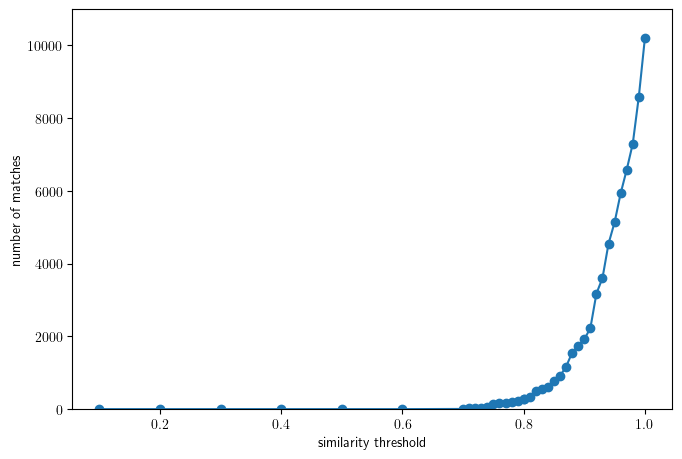
\includegraphics[width=\textwidth]{countries_20-most-popul_thresholds.png}
%         \caption{Similarity threshold variation for all \textsf{semsim} patterns}
%         \label{fig:countries_20-most-popul_thresholds}
%     \end{subfigure}
%     \begin{subfigure}[t]{0.9\textwidth}
%         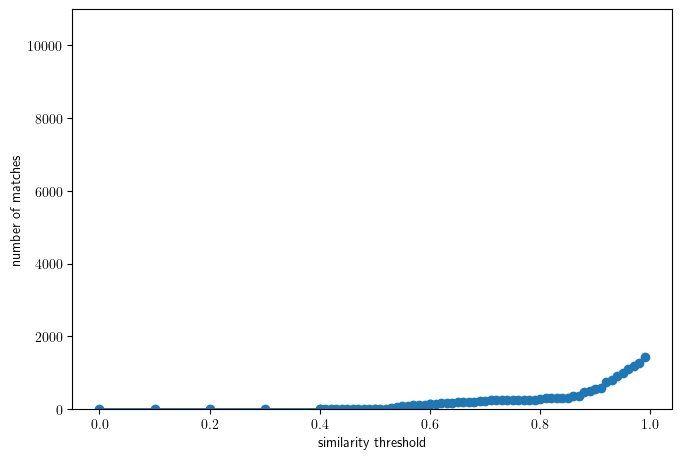
\includegraphics[width=\textwidth]{countries_20-most-popul_thresholds-countries.png}
%         \caption{Similarity threshold variation only for \textsf{SOURCE} and \textsf{TARGET} (country) \texttt{semsim} patterns}
%         \label{fig:countries_20-most-popul_thresholds-countries}
%     \end{subfigure}
%\caption{Number of matches for conflict pattern in relation to similarity threshold}
%\label{fig:case-study-conflict-countries-1}   
%\end{figure}
%
%\begin{figure}
%     \centering
%     \begin{subfigure}[t]{0.9\textwidth}
%         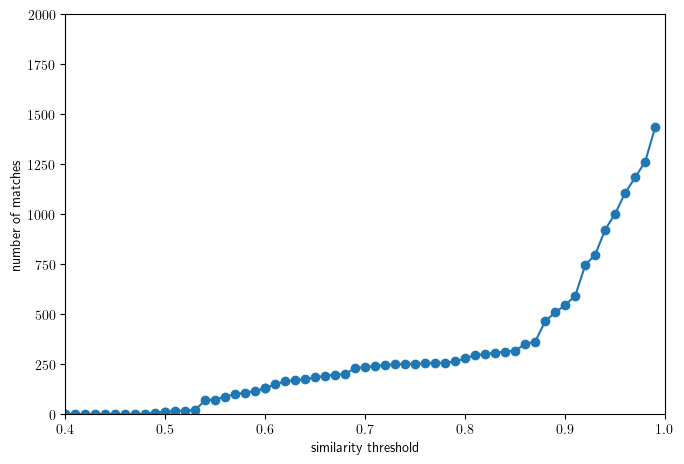
\includegraphics[width=\textwidth]{countries_20-most-popul_thresholds-countries_greater-0.4.png}
%     \end{subfigure}
%\caption{Number of matches for conflict pattern in relation to similarity threshold with threshold variation for \textsf{SOURCE} and \textsf{TARGET} (i.e. COUNTRIES) \texttt{semsim} patterns in the range \(0.4 >=\) threshold \(< 1.0\) (and y-axis limited to 2000 results)}
%\label{fig:case-study-conflict-countries-2}   
%\end{figure}

\subsection{Qualitative Results}


\begin{sidewaystable}
%    \centering
    \caption{hyper dyper table}

\begin{tabular}{L{4cm}L{2cm}L{5cm}L{3cm}L{5cm}L{3cm}}
\toprule
Scenario Name & Pattern & Samples & Variable Threshold & Reference Edges & Ref. Edges Source \\
\midrule
1\_original-pattern & Pattern X & Erdogan slams ridicule of 'Muslims discovered Americas' claim\newline Iran forces 'kill Kurdish rebels on Iraq border\newline Ukraine Accuses Russia of Invasion & -/- & -/- & -/- \\
2-1\_semsim-fix\_preds & Pattern X & Pakistani police kill feared militant leader in mysterious pre-dawn shootout\newline Al-Shabaab militants claim responsibility for deadly attack on Garissa University College in Kenya\newline Casualties as Congo troops, UN forces fight rebels & 'preds': 0.19\newline Percentile: 50 & -/- & -/- \\
2-2\_semsim-fix\_preps & Pattern X & Iranian police have arrested merchants for selling clothing that featured the flags of the United States and Britain, two longtime foes of the Islamic republic\newline Syrian Air Force Strikes kill 38 ISIS fighters\newline Seven Libyan soldiers killed fighting off Islamists near Benghazi: source & 'preps': 0.54\newline Percentile: 50 & -/- & -/- \\
\bottomrule
\end{tabular}

\end{sidewaystable}

%\begin{table*}
%\
%\end{table*}

% ========== 
\chapter{Conclusion}

\chapter{Future Work}
\section{Implementation Improvements}
implemnt multiprocessing, i.e. server process for both hypergraph and semsim matchers. other option would be to leverage python shared memory capabilities but is likely to be less stable and has less scaling potential





\printbibliography


\end{document}
